\documentclass[12pt]{article}
\usepackage[utf8]{inputenc}
\usepackage[english]{babel}
\usepackage{pgfplots}

\pgfplotsset{compat=1.9}

\begin{document}

\title{Cascaded Approximation of Gaussian Blur}
\author{Vabishchevich Nikolay}
\date{May 8, 2015}
\maketitle


\section{Test Graph}

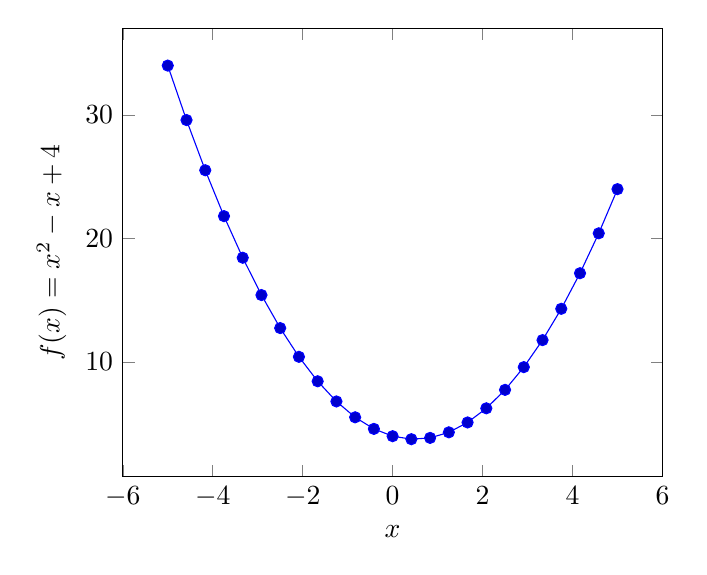
\begin{tikzpicture}
	\begin{axis}[
		xlabel=$x$,
		ylabel={$f(x) = x^2 - x +4$}
	]
	% use TeX as calculator:
	\addplot {x^2 - x +4};
	\end{axis}
\end{tikzpicture}

\begin{tikzpicture}
	\begin{axis}[
		xlabel=$x$,
		ylabel=$\sin(x)$
	]
	% invoke external gnuplot as
	% calculator:
	\addplot gnuplot[id=sin]{sin(x)};
	\end{axis}
\end{tikzpicture}

\end{document}
